\documentclass{article}
\usepackage{amsmath}
\usepackage{hyperref}
\usepackage{tikz}
\usetikzlibrary{calc,arrows,shapes,positioning}
\usepackage{tkz-euclide}
\usepackage{float}
\usepackage{xstring}
\usepackage{catchfile}
\usepackage{siunitx}

\CatchFileDef{\headfull}{../.git/HEAD}{}
\StrGobbleRight{\headfull}{1}[\head]
\StrBehind[2]{\head}{/}[\branch]
\IfFileExists{../.git/refs/heads/\branch}{%
    \CatchFileDef{\commit}{../.git/refs/heads/\branch}{}}{%
    \newcommand{\commit}{\dots~(in \emph{packed-refs})}}
\newcommand{\gitrevision}{%
  \StrLeft{\commit}{7}%
}

\title{Codec 2}
\author{David Rowe\\ \\ Revision: {\gitrevision} on branch: {\branch}}

\begin{document}

% Tikz code used to support block diagrams
% credit: https://tex.stackexchange.com/questions/175969/block-diagrams-using-tikz

\tikzset{
block/.style = {draw, fill=white, rectangle, minimum height=3em, minimum width=3em},
tmp/.style  = {coordinate}, 
circ/.style= {draw, fill=white, circle, node distance=1cm, minimum size=0.6cm},
input/.style = {coordinate},
output/.style= {coordinate},
pinstyle/.style = {pin edge={to-,thin,black}}
}

% tikz: draws a sine wave
\newcommand{\drawSine}[4]{% x, y, x_scale, y_scale

\draw plot [smooth] coordinates {(#1-2*#3, #2 )       (#1-1.5*#3,#2+0.707*#4)
                                 (#1-1*#3, #2+1*#4)   (#1-0.5*#3,#2+0.707*#4)
                                 (#1  ,#2+0)          (#1+0.5*#3,#2-0.707*#4) 
                                 (#1+1*#3,#2-1*#4)    (#1+1.5*#3,#2-0.707*#4)
                                 (#1+2*#3,#2+0)}
}

% tikz: draw a summer
\newcommand{\drawSummer}[2]{% x, y
	\draw (#1,#2) circle (0.5);
	\draw (#1-0.25,#2) -- (#1+0.25,#2);
	\draw (#1,#2-0.25) -- (#1,#2+0.25);
}

\maketitle

\section{Introduction}

Codec 2 is an open source speech codec designed for communications quality speech between 700 and 3200 bit/s. The main application is low bandwidth HF/VHF digital radio. It fills a gap in open source voice codecs beneath 5000 bit/s and is released under the GNU Lesser General Public License (LGPL).

Key feature includes:
\begin{enumerate}
\item A range of modes supporting different bit rates, currently (Nov 2023): 3200, 2400, 1600, 1400, 1300, 1200, 700C.  The number is the bit rate, and the supplementary letter the version (700C replaced the earlier 700, 700A, 700B versions). These are referred to as ``Codec 2 3200", ``Codec 2 700C" etc.
\item Modest CPU (a few 10s of MIPs) and memory (a few 10s of kbytes of RAM) requirements such that it can run on stm32 class microcontrollers with hardware FPU.
\item Codec 2 has been designed for digital voice over radio applications, and retains intelligible speech at a few percent bit error rate.
\item An open source reference implementation in the C language for C99/gcc compilers, and a \emph{cmake} build and test framework that runs on Linux.  Also included is a cross compiled stm32 reference implementation.
\item Ports to non-C99 compilers (e.g. MSVC, some microcontrollers, native builds on Windows) are left to third party developers - we recommend the tests also be ported and pass before considering the port successful.
\end{enumerate}

The Codec 2 project was started in 2009 in response to the problem of closed source, patented, proprietary voice codecs in the sub-5 kbit/s range, in particular for use in the Amateur Radio service.

This document describes Codec 2 at two levels.  Section \ref{sect:overview} is a high level description aimed at the Radio Amateur, while Section \ref{sect:details} contains a more detailed description using math and signal processing theory.  Combined with the C source code, it is intended to give the reader enough information to understand the operation of Codec 2 in detail and embark on source code level projects, such as improvements, ports to other languages, student or academic research projects.  Issues with the current algorithms and topics for further work are also included.  Section {\ref{sect:codec2_modes} provides a summary of the Codec 2 modes, and Section \ref{sect:source_files} a guide to the C source files.  A glossary of terms and symbols is provided in Section \ref{sect:glossary}, and Section \ref{sect:further_work} has suggestions for further documentation work.

This production of this document was kindly supported by an ARDC grant \cite{ardc2023}.  As an open source project, many people have contributed to Codec 2 over the years - we deeply appreciate all of your support.

\section{Codec 2 for the Radio Amateur}
\label{sect:overview}

\subsection{Model Based Speech Coding}

A speech codec takes speech samples from an A/D converter (e.g. 16 bit samples at 8 kHz or 128 kbits/s) and compresses them down to a low bit rate that can be more easily sent over a narrow bandwidth channel (e.g. 700 bits/s for HF).  Speech coding is the art of ``what can we throw away". We need to lower the bit rate of the speech while retaining speech you can understand, and making it sound as natural as possible.

As such low bit rates we use a speech production ``model".  The input speech is analysed, and we extract model parameters, which are then sent over the channel.  An example of a model based parameter is the pitch of the person speaking.  We estimate the pitch of the speaker, quantise it to a 7 bit number, and send that over the channel every 20ms.

The model based approach used by Codec 2 allows high compression, with some trade offs such as noticeable artefacts in the decoded speech.  Higher bit rate codecs (above 5000 bit/s), such as those use for mobile telephony or voice on the Internet, tend to pay more attention to preserving the speech waveform, or use a hybrid approach of waveform and model based techniques.  They sound better but require a higher bit rate.

Recently, machine learning has been applied to speech coding.  This technology promises high quality, artefact free speech quality at low bit rates, but currently (2023) requires significantly more memory and CPU resources than traditional speech coding technology such as Codec 2.  However the field is progressing rapidly, and as the cost of CPU and memory decreases (Moore's law) will soon be a viable technology for many low bit rate speech applications.

\subsection{Speech in Time and Frequency}

To explain how Codec 2 works, lets look at some speech. Figure \ref{fig:hts2a_time} shows a short 40ms segment of speech in the time and frequency domain.  On the time plot we can see the waveform is changing slowly over time as the word is articulated.  On the right hand side it also appears to repeat itself - one cycle looks very similar to the last.  This cycle time is the ``pitch period", which for this example is around $P=35$ samples.  Given we are sampling at $F_s=8000$ Hz, the pitch period is $P/F_s=35/8000=0.0044$ seconds, or 4.4ms.

\begin{figure} [H]
\caption{ A 40ms segment from the word ``these" from a female speaker, sampled at 8kHz. Top is a plot against time, bottom (blue) is a plot of the same speech against frequency. The waveform repeats itself every 4.3ms ($F_0=230$ Hz), this is the ``pitch period" of this segment.  The red crosses are the sine wave amplitudes, explained in the text.}
\label{fig:hts2a_time}
\begin{center}
\input hts2a_37_sn.tex
\\
\input hts2a_37_sw.tex
\end{center}
\end{figure}

Now if the pitch period is 4.4ms, the pitch frequency or \emph{fundamental} frequency $F_0$ is about $1/0.0044 \approx 230$ Hz.  If we look at the blue frequency domain plot at the bottom of Figure \ref{fig:hts2a_time}, we can see spikes that repeat every 230 Hz.  If the signal is repeating itself in the time domain, it also repeats itself in the frequency domain.  Those spikes separated by about 230 Hz are harmonics of the fundamental frequency $F_0$.

Note that each harmonic has it's own amplitude, that varies across frequency.  The red line plots the amplitude of each harmonic. In this example there is a peak around 500 Hz, and another, broader peak around 2300 Hz.  The ear perceives speech by the location of these peaks and troughs.

\subsection{Sinusoidal Speech Coding}

A sinewave will cause a spike or spectral line on a spectrum plot, so we can see each spike as a small sine wave generator.  Each sine wave generator has it's own frequency that are all multiples of the fundamental pitch frequency (e.g. $230, 460, 690,...$ Hz).  They will also have their own amplitude and phase.  If we add all the sine waves together (Figure \ref{fig:sinusoidal_model}) we can produce reasonable quality synthesised speech.  This is called sinusoidal speech coding and is the speech production ``model" at the heart of Codec 2.

\begin{figure}[h]
\caption{The sinusoidal speech model.  If we sum a series of sine waves, we can generate a speech signal.  Each sinewave has it's own amplitude ($A_1,A_2,... A_L$), frequency, and phase (not shown).  We assume the frequencies are multiples of the fundamental frequency $F_0$. $L$ is the total number of sinewaves we can fit in 4 kHz.}
\label{fig:sinusoidal_model}
\begin{center}
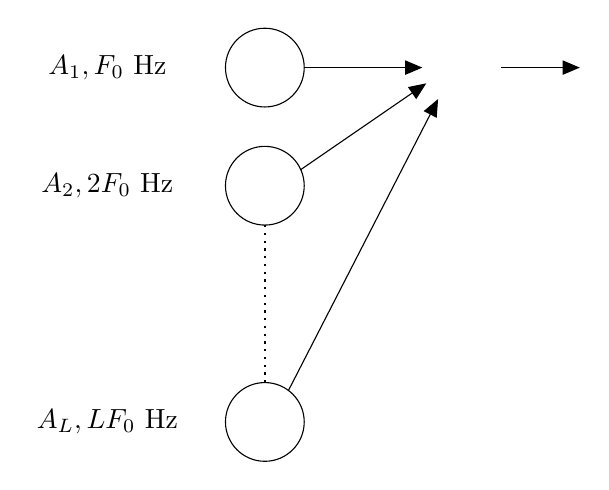
\begin{tikzpicture}[>=triangle 45,x=1.0cm,y=1.0cm]

% sine wave sources
\draw (0, 2.0) circle (0.5); \drawSine{0}{ 2.0}{0.2}{0.2}; \draw (-2.0,2.0) node {$A_1, F_0$ Hz};
\draw (0, 0.5) circle (0.5); \drawSine{0}{ 0.5}{0.2}{0.2}; \draw (-2.0,0.5) node {$A_2, 2F_0$ Hz};
\draw (0,-2.5) circle (0.5); \drawSine{0}{-2.5}{0.2}{0.2}; \draw (-2.0,-2.5) node {$A_L, LF_0$ Hz};
\draw [dotted,thick] (0,0) -- (0,-2);

\drawSummer{2.5}{2};

% connecting lines
\draw [->] (0.5,2) -- (2,2);
\draw [->] (0.45,0.7) -- (2.05,1.8);
\draw [->] (0.3,-2.1) -- (2.2,1.6);

% output speech
\draw [->] (3,2) -- (4,2);
\draw [xshift=4.2cm,yshift=2cm,color=blue] plot[smooth] file {hts2a_37_sn.txt};

\end{tikzpicture}
\end{center}
\end{figure}

The model parameters evolve over time, but can generally be considered constant for a short time window (a few 10s of ms).  For example pitch evolves over time, moving up or down as a word is articulated.

As the model parameters change over time, we need to keep updating them.  This is known as the \emph{frame rate} of the codec, which can be expressed in terms of frequency (Hz) or time (ms).  For sampling model parameters Codec 2 uses a frame rate of 10ms.  For transmission over the channel we reduce this to 20-40ms, in order to lower the bit rate.  The trade off with a lower frame rate is reduced speech quality.

The parameters of the sinusoidal model are:
\begin{enumerate}
\item The frequency of each sine wave.  As they are all harmonics of $F_0$ we can just send $F_0$ to the decoder, and it can reconstruct the frequency of each harmonic as $F_0,2F_0,3F_0,...,LF_0$.  We used 5-7 bits/frame to represent $F_0$ in Codec 2.
\item The amplitude of each sine wave, $A_1,A_2,...,A_L$.  These ``spectral amplitudes" are really important as they convey the information the ear needs to understand speech.  Most of the bits are used for spectral amplitude information.  Codec 2 uses between 18 and 50 bits/frame for spectral amplitude information.
\item Voicing information.  Speech can be approximated into voiced speech (vowels) and unvoiced speech (like consonants), or some mixture of the two.  The example in Figure \ref{fig:hts2a_time} above is voiced speech.  So we need some way to describe voicing to the decoder. This requires just a few bits/frame.
\item The phase of each sine wave.  Codec 2 discards the phases of each harmonic at the encoder and reconstruct them at the decoder using an algorithm, so no bits are required for phases.  This results in some drop in speech quality.
\end{enumerate}

\subsection{Codec 2 Encoder and Decoder}

This section explains how the Codec 2 encoder and decoder works using block diagrams.

\begin{figure}[h]
\caption{Codec 2 Encoder.}
\label{fig:codec2_encoder}
\begin{center}
\begin{tikzpicture}[auto, node distance=2cm,>=triangle 45,x=1.0cm,y=1.0cm,align=center,text width=2cm]

\node [input] (rinput) {};
\node [input, right of=rinput,node distance=0.5cm] (z) {};
\node [block, right of=z,node distance=1.5cm] (pitch_est) {Pitch Estimator};
\node [block, below of=pitch_est] (fft) {FFT};
\node [block, right of=fft,node distance=3cm] (est_am) {Estimate Amplitudes};
\node [block, below of=est_am] (est_v) {Estimate Voicing};
\node [block, right of=est_am,node distance=3cm] (quant) {Decimate Quantise};
\node [output, right of=quant,node distance=2cm] (routput) {};

\draw [->] node[align=left] {Input Speech} (rinput) --  (pitch_est);
\draw [->] (z) |- (fft);
\draw [->] (pitch_est) -| (est_am);
\draw [->] (fft) -- (est_am);
\draw [->] (est_am) -- (est_v);
\draw [->] (pitch_est) -| (quant);
\draw [->] (est_am) -- (quant);
\draw [->] (est_v) -| (quant);
\draw [->] (est_v) -| (quant); 
\draw [->] (quant) -- (routput) node[right, align=left, text width=1.5cm] {Bit Stream};

\end{tikzpicture}
\end{center}
\end{figure}

The encoder is presented in Figure \ref{fig:codec2_encoder}.  Frames of input speech samples are passed to a Fast Fourier Transform (FFT), which converts the time domain samples to the frequency domain.  The same frame of input samples is used to estimate the pitch of the current frame. We then use the pitch and frequency domain speech to estimate the amplitude of each sine wave.

Yet another algorithm is used to determine if the frame is voiced or unvoiced.  This works by comparing the spectrum to what we would expect for voiced speech (e.g. lots of spectral lines).  If the energy is more random and continuous rather than discrete lines, we consider it unvoiced.

Up until this point the processing happens at a 10ms frame rate.  However in the next step we ``decimate`` the model parameters - this means we discard some of the model parameters to lower the frame rate, which helps us lower the bit rate.  Decimating to 20ms (throwing away every 2nd set of model parameters) doesn't have much effect, but beyond that the speech quality starts to degrade.  So there is a trade off between decimation rate and bit rate over the channel.

Once we have the desired frame rate, we ``quantise" each model parameter.  This means we use a fixed number of bits to represent it, so we can send the bits over the channel.  Parameters like pitch and voicing are fairly easy, but quite a bit of DSP goes into quantising the spectral amplitudes. For the higher bit rate Codec 2 modes, we design a filter that matches the spectral amplitudes, then send a quantised version of the filter over the channel. Using the example in Figure \ref{fig:hts2a_time} - the filter would have a band pass peaks at 500 and 2300 Hz.  It's frequency response would follow the red line. The filter is time varying - we redesign it for every frame.

You'll notice the term ``estimate" being used a lot.  One of the problems with model based speech coding is the algorithms we use to extract the model parameters are not perfect.  Occasionally the algorithms get it wrong.  Look at the red crosses on the bottom plot of Figure \ref{fig:hts2a_time}.  These mark the amplitude estimate of each harmonic.  If you look carefully, you'll see that above 2000Hz, the crosses fall a little short of the exact centre of each harmonic.  This is an example of a ``fine" pitch estimator error, a little off the correct value.

Often the errors interact, for example the fine pitch error shown above will mean the amplitude estimates are a little bit off as well. Fortunately these errors tend to be temporary, and are sometimes not even noticeable to the listener - remember this codec is often used for HF/VHF radio where channel noise is part of the normal experience.
 
\begin{figure}[h]
\caption{Codec 2 Decoder}
\label{fig:codec2_decoder}
\begin{center}
\begin{tikzpicture}[auto, node distance=2cm,>=triangle 45,x=1.0cm,y=1.0cm,align=center,text width=2cm]

\node [input] (rinput) {};
\node [block, right of=rinput,node distance=2cm] (dequantise) {Dequantise Interpolate};
\node [block, right of=dequantise,node distance=3cm] (recover) {Recover Amplitudes};
\node [block, right of=recover,node distance=3cm] (synthesise) {Synthesise Speech};
\node [block, above of=synthesise] (phase) {Synthesise Phases};
\node [output, right of=synthesise,node distance=2cm] (routput) {};

\draw [->] node[align=left, text width=1.5cm] {Bit Stream} (rinput) --  (dequantise);
\draw [->] (dequantise) -- (recover);
\draw [->] (recover) -- (synthesise);
\draw [->] (recover) |- (phase);
\draw [->] (phase) -- (synthesise);
\draw [->] (synthesise) -- (routput) node[right, align=left, text width=1.5cm] {Output Speech};

\end{tikzpicture}
\end{center}
\end{figure}

Figure \ref{fig:codec2_decoder} shows the operation of the Codec 2 decoder.  We take the sequence of bits received from the channel and recover the quantised model parameters, pitch, spectral amplitudes, and voicing.  We then resample the model parameters back up to the 10ms frame rate using a technique called interpolation.  For example say we receive a $F_0=200$ Hz pitch value then 20ms later $F_0=220$ Hz.  We can use the average $F_0=210$ Hz for the middle 10ms frame.

The phases of each harmonic are generated using the other model parameters and some DSP.  It turns out that if you know the amplitude spectrum, you can determine a ``reasonable" phase spectrum using some DSP operations, which in practice is implemented with a couple of FFTs.  We also use the voicing information - for unvoiced speech we use random phases (a good way to synthesise noise-like signals) - and for voiced speech we make sure the phases are chosen so the synthesised speech transitions smoothly from one frame to the next.

Frames of speech are synthesised using an inverse FFT.  We take a blank array of FFT samples, and at intervals of $F_0$ insert samples with the amplitude and phase of each harmonic.  We then inverse FFT to create a frame of time domain samples.  These frames of synthesised speech samples are carefully aligned with the previous frame to ensure smooth frame-frame transitions, and output to the listener.

\subsection{Bit Allocation}

Table \ref{tab:bit_allocation} presents the bit allocation for two popular Codec 2 modes.  One additional parameter is the frame energy, this is the average level of the spectral amplitudes, or ``AF gain" of the speech frame.

At very low bit rates such as 700 bits/s, we use Vector Quantisation (VQ) to represent the spectral amplitudes.  We construct a table such that each row of the table has a set of spectral amplitude samples.  In Codec 2 700C the table has 512 rows.  During the quantisation process, we choose the table row that best matches the spectral amplitudes for this frame, then send the \emph{index} of the table row.  The decoder has a similar table, so can use the index to look up the spectral amplitude values.  If the table is 512 rows, we can use a 9 bit number to quantise the spectral amplitudes.  In Codec 2 700C, we use two tables of 512 entries each (18 bits total), the second one helps fine tune the quantisation from the first table.

Vector Quantisation can only represent what is present in the tables, so if it sees anything unusual (for example a different microphone frequency response or background noise), the quantisation can become very rough and speech quality poor.  We train the tables at design time using a database of speech samples and a training algorithm - an early form of machine learning.

Codec 2 3200 uses the method of fitting a filter to the spectral amplitudes, this approach tends to be more forgiving of small variations in the input speech spectrum, but is not as efficient in terms of bit rate.

\begin{table}[H]
\label{tab:bit_allocation}
\centering
\begin{tabular}{l c c }
\hline
Parameter & 3200 & 700C \\
\hline
Pitch $F_0$ & 7 & 5 \\
Spectral Amplitudes $\{A_m\}$ & 50 & 18 \\
Energy & 5 & 3 \\
Voicing & 2 & 1 \\
Bits/frame & 64 & 28 \\
Frame Rate & 20ms & 40ms \\
Bit rate & 3200 & 700 \\
\hline
\end{tabular}
\caption{Bit allocation of the 3200 and 700C modes}
\end{table}

\section{Detailed Design}
\label{sect:details}

\subsection{Overview}

Codec 2 is based on sinusoidal \cite{mcaulay1986speech} and Multi-Band Excitation (MBE) \cite{griffin1988multiband} vocoders that were first developed in the late 1980s.  Descendants of the MBE vocoders (IMBE, AMBE etc) have enjoyed widespread use in many applications such as VHF/UHF hand held radios and satellite communications. In the 1990s the author studied sinusoidal speech coding \cite{rowe1997techniques}, which provided the skill set and a practical, patent free baseline for starting the Codec 2 project:

Some features of the Codec 2 Design:
\begin{enumerate}
\item A pitch estimator based on a 2nd order non-linearity developed by the author.
\item A single voiced/unvoiced binary voicing model.
\item A frequency domain IFFT/overlap-add synthesis model for voiced and unvoiced speech.
\item Phases are not transmitted, they are synthesised at the decoder from the magnitude spectrum and voicing decision.  
\item For the higher bit rate modes (1200 to 3200 bits/s), spectral magnitudes are represented using LPCs extracted from time domain analysis and scalar LSP quantisation.
\item For Codec 2 700C, vector quantisation of resampled spectral magnitudes in the log domain.
\item Minimal interframe prediction in order to minimise error propagation and maximise robustness to channel errors.
\item A post filter that enhances the speech quality of the baseline codec, especially for low pitched (male) speakers.
\end{enumerate}

\subsection{Sinusoidal Analysis}

Both voiced and unvoiced speech is represented using a harmonic sinusoidal model:
\begin{equation}
\hat{s}(n) = \sum_{m=1}^L A_m cos(\omega_0 m n + \theta_m)
\end{equation}
where the parameters $A_m, \theta_m, m=1...L$ represent the magnitude and phases of each sinusoid, $\omega_0$ is the fundamental frequency in radians/sample, and $L=\lfloor \pi/\omega_0 \rfloor$ is the number of harmonics.

Figure \ref{fig:analysis} illustrates the processing steps in the sinusoidal analysis system at the core of the Codec 2 encoder.  This algorithms described in this section are based on the work in \cite{rowe1997techniques}, with some changes in notation.

\begin{figure}[h]
\caption{Sinusoidal Analysis}
\label{fig:analysis}
\begin{center}
\begin{tikzpicture}[auto, node distance=2cm,>=triangle 45,x=1.0cm,y=1.0cm, align=center]

\node [input] (rinput) {};
\node [tmp, right of=rinput,node distance=0.5cm] (z) {};
\node [block, right of=z,node distance=1.5cm] (window) {Window};
\node [block, right of=window,node distance=2.5cm] (dft) {DFT};
\node [block, right of=dft,node distance=3cm,text width=2cm] (est) {Est Amp and Phase};
\node [block, below of=window] (nlp) {NLP};
\node [output, right of=est,node distance=2cm] (routput) {};

\draw [->] node[align=left,text width=2cm] {$s(n)$} (rinput) -- (window);
\draw [->] (z) |- (nlp);
\draw [->] (window) -- node[below] {$s_w(n)$} (dft);
\draw [->] (dft) -- node[below] {$S_\omega(k)$} (est);
\draw [->] (nlp) -| node[below] {$\omega_0$} (est) ;
\draw [->] (est) -- (routput) node[right] {$\{A_m\}$ \\ $\{\theta_m\}$};

\end{tikzpicture}
\end{center}
\end{figure}

The time domain speech signal $s(n)$ is divided into overlapping analysis windows (frames) of $N_w=279$ samples. The centre of each analysis window is separated by $N=80$ or 10ms. Codec 2 operates at an internal frame rate of 100 Hz. To analyse the $l$-th frame it is convenient to convert the fixed time reference to a sliding time reference centred on the current analysis window:
\begin{equation}
s_w(n) = s(lN + n) w(n), \quad n = - N_{w2} ... N_{w2}
\end{equation}
where $w(n)$ is a tapered even window of $N_w$ ($N_w$ odd) samples with:
\begin{equation}
N_{w2} = \left \lfloor \frac{N_w}{2} \right \rfloor
\end{equation}
A suitable window function is a shifted Hann window:
\begin{equation}
w(n) = \frac{1}{2} - \frac{1}{2} cos \left(\frac{2 \pi (n- N_{w2})}{N_w-1} \right)
\end{equation}
where the energy in the window is normalised such that:
\begin{equation}
\sum_{n=0}^{N_w-1}w^2(n) = \frac{1}{N_{dft}}
\end{equation}
To analyse $s(n)$ in the frequency domain the $N_{dft}$ point Discrete Fourier Transform (DFT) can be computed:
\begin{equation}
S_w(k) = \sum_{n=-N_{w2}}^{N_{w2}} s_w(n) e^{-j 2 \pi k n / N_{dft}}
\end{equation}
The magnitude and phase of each harmonic is given by:
\begin{equation}
\label{eq:mag_est}
A_m = \sqrt{\sum_{k=a_m}^{b_m-1} |S_w(k)|^2 }
\end{equation}
\begin{equation}
\theta_m = arg \left[ S_w(\lfloor m r \rceil \right]
\end{equation}
where:
\begin{equation}
\begin{split}
a_m      &= \lfloor (m - 0.5)r \rceil \\
b_m      &= \lfloor (m + 0.5)r \rceil \\
r        &= \frac{\omega_0 N_{dft}}{2 \pi} 
\end{split}
\end{equation}
The DFT indexes $a_m, b_m$ select the band of $S_w(k)$ containing the $m$-th harmonic; $r$ maps the harmonic number $m$ to the nearest DFT index, and $\lfloor x \rceil$ is the rounding operator. This method of estimating $A_m$ is relatively insensitive to small errors in $F0$ estimation and works equally well for voiced and unvoiced speech.  Figure $\ref{fig:hts2a_time}$ plots $S_w$ (blue) and $\{A_m\}$ (red) for a sample frame of female speech.

The phase is sampled at the centre of the band.  For all practical Codec 2 modes the phase is not transmitted to the decoder so does not need to be computed.  However speech synthesised using the phase is useful as a control during development, and is available using the \emph{c2sim} utility.

\subsection{Sinusoidal Synthesis}

Synthesis is achieved by constructing an estimate of the original speech spectrum using the sinusoidal model parameters for the current frame. This information is then transformed to the time domain using an Inverse DFT (IDFT). To produce a continuous time domain waveform the IDFTs from adjacent frames are smoothly interpolated using a weighted overlap add procedure \cite{mcaulay1986speech}.

\begin{figure}[h]
\caption{Sinusoidal Synthesis.  At frame $l$ the windowing function generates $2N$ samples.  The first $N$ samples complete the current frame. The second $N$ samples are stored for summing with the next frame.}
\label{fig:synthesis}
\begin{center}
\begin{tikzpicture}[auto, node distance=2cm,>=triangle 45,x=1.0cm,y=1.0cm, align=center]

\node [input] (rinput) {};
\node [block, right of=rinput,node distance=1.5cm,text width=1.5cm] (construct) {Construct $S_w(k)$};
\node [block, right of=construct,node distance=2cm] (idft) {IDFT};
\node [block, right of=idft,node distance=2.5cm,text width=1.5cm] (window) {Window $t(n)$};
\node [circ, right of=window,node distance=3cm] (sum) {$+$};
\node [block, below of=sum,text width=1.5cm] (delay) {1 frame delay};
\node [output, right of=sum,node distance=1cm] (routput) {};

\draw [->] node[left of=rinput,node distance=0.5cm] {$\omega_0$\\$\{A_m\}$\\$\{\theta_m\}$} (rinput) -- (construct);
\draw [->] (construct) --(idft);
\draw [->] (idft) --  node[below] {$\hat{s}_l(n)$} (window);
\draw [->] (window) -- node[above of=window, node distance=0.75cm] 
  {$\begin{aligned} n =& 0,..,\\[-0.5ex] & N-1 \end{aligned}$} (sum);
\draw [->] (window) |-  (delay)  node[left of=delay,below, node distance=2cm] 
  {$\begin{aligned} n =& N,...,\\[-0.5ex] & 2N-1 \end{aligned}$};
\draw [->] (delay) -- (sum);
\draw [->] (sum) -- (routput) node[right] {$\hat{s}(n+lN)$};

\end{tikzpicture}
\end{center}
\end{figure}

The synthetic speech spectrum is constructed using the sinusoidal model parameters by populating a DFT array $\hat{S}_w(k)$ with weighted impulses at the harmonic centres:
\begin{equation}
\hat{S}_w(k) = \begin{cases}
                A_m e^{j\theta_m}, & k = \lfloor m r \rceil, m=1..L \\
                0, & otherwise
                \end{cases}
\end{equation}

As we wish to synthesise a real time domain signal, $S_w(k)$ is defined to be conjugate symmetric:
\begin{equation}
\hat{S}_w(N_{dft}-k) = \hat{S}_w^{*}(k), \quad k = 1,.. N_{dft}/2-1
\end{equation}
where $\hat{S}_w^*(k)$ is the complex conjugate of $\hat{S}_w(k)$. This signal is converted to the time domain
using the IDFT:
\begin{equation}
\label{eq:synth_idft}
\hat{s}_l(n) = \frac{1}{N_{dft}}\sum_{k=0}^{N_{dft}-1} \hat{S}_w(k) e^{j 2 \pi k n / N_{dft}}
\end{equation}
Where $N_{dft} > 2N$, to support the overlap add procedure below.

We introduce the notation $\hat{s}_l(n)$ to denote the synthesised speech for the $l$-th frame. To reconstruct a continuous synthesised speech waveform, we need to smoothly connect adjacent synthesised frames of speech. This is performed by windowing each frame of synthesised speech, then shifting and superimposing adjacent frames using an overlap add algorithm. A triangular window is defined by:
\begin{equation}
t(n) = \begin{cases}
          n/N,         & 0 \le n < N  \\
          1 - (n-N)/N, & N \le n < 2N \\ 
          0,           & otherwise
       \end{cases}
\end{equation}
The frame size, $N=80$, is the same as the encoder. The shape and overlap of the synthesis window is not important, as long as sections separated by the frame size (frame to frame shift) sum to 1:
\begin{equation}
t(n) + t(N-n) = 1
\end{equation}
The continuous synthesised speech signal $\hat{s}(n)$ for the $l$-th frame is obtained using:
\begin{equation}
\hat{s}(n+lN) = \begin{cases}
                    \hat{s}(n+(l-1)N) + \hat{s}_l(N_{dft}-N+1+n)t(n), & n=0,1,...,N-2 \\ 
		            \hat{s}_l(n - N - 1)t(n)                                    & n=N-1,..,2N-1
                  \end{cases}
\end{equation}

From the $N_{dft}$ samples produced by the IDFT (\ref{eq:synth_idft}), after windowing we have $2N$ output samples. The first $N$ output samples $n=0,...N-1$ complete the current frame $l$ and are output from the synthesiser.  However we must also compute the contribution to the next frame $n = N,N+1,...,2N-1$.  These are stored, and added to samples from the next synthesised frame.

\subsection{Non-Linear Pitch Estimation}
\label{sect:nlp}

The Non-Linear Pitch (NLP) pitch estimator was developed by the author, described in detail in chapter 4 of \cite{rowe1997techniques}, and portions of this description are reproduced here.  The post processing algorithm used for pitch estimation in Codec 2 is different from \cite{rowe1997techniques} and is described here.  The C code \emph{nlp.c} is a useful reference for the fine details of the implementation, and the Octave script \emph{plnlp.m} can by used to plot the internal states and single step through speech, illustrating the operation of the algorithm.

The core pitch detector is based on a square law non-linearity, that is applied directly to the input speech signal. Given speech is composed of harmonics separated by $F_0$ the non-linearity generates intermodulation products at $F_0$, even if the fundamental is absent from the input signal due to high pass filtering.

Figure \ref{fig:nlp} illustrates the algorithm. The fundamental frequency $F_0$ is estimated in the range of 50-400 Hz. The algorithm is designed to take blocks of $M = 320$ samples at a sample rate of 8 kHz (40 ms time window). This block length ensures at least two pitch periods lie within the analysis window at the lowest fundamental frequency.

The speech signal is first squared then notch filtered to remove the DC component from the squared time domain signal. This prevents the large amplitude DC term from interfering with the somewhat smaller amplitude term at the fundamental. This is particularly important for male speakers, who may have low frequency fundamentals close to DC. The notch filter is applied in the time domain and has the experimentally derived transfer function:
\begin{equation}
H_{notch}(z) = \frac{1-z^{-1}}{1-0.95z^{-1}}
\end{equation}

\begin{figure}[h]
\caption{The Non-Linear Pitch (NLP) algorithm}
\label{fig:nlp}
\begin{center}
\begin{tikzpicture}[auto, node distance=2cm,>=triangle 45,x=1.0cm,y=1.0cm, align=center]

\node [input] (rinput) {};
\node [tmp, right of=rinput,node distance=0.5cm] (z) {};
\node [tmp, below of=z,node distance=1cm] (z1) {};
\node [circ, right of=z,node distance=1cm] (mult) {$\times$};
\node [block, right of=mult,node distance=2cm,text width=2cm] (notch) {DC Notch Filter};
\node [block, right of=notch,node distance=3cm,text width=2cm] (lpf) {Low Pass Filter};
\node [block, right of=lpf,node distance=2.5cm] (dec5) {$\downarrow 5$};
\node [block, below of=dec5] (dft) {DFT};
\node [block, below of=lpf] (peak) {Peak Pick};
\node [block, below of=notch,text width=2cm] (search) {Sub \\Multiple Search};
\node [block, left of=search,node distance=3cm] (refine) {Refinement};
\node [output, left of=refine,node distance=2cm] (routput) {};

\draw [->] node[align=left,text width=2cm] {Input Speech} (rinput) -- (mult);
\draw [->] (z) -- (z1) -| (mult);
\draw [->] (mult) -- (notch);
\draw [->] (notch) -- (lpf);
\draw [->] (lpf) -- (dec5);
\draw [->] (dec5) -- (dft);
\draw [->] (dft) -- (peak);
\draw [->] (peak) -- (search);
\draw [->] (search) -- (refine);
\draw [->] (refine) -- (routput) node[left, align=center] {$F_0$};

\end{tikzpicture}
\end{center}
\end{figure}

Before transforming the squared signal to the frequency domain, the signal is low pass filtered and decimated by a factor of 5. This operation is performed to limit the bandwidth of the squared signal to the approximate range of the fundamental frequency. All energy in the squared signal above 400 Hz is superfluous and would lower the resolution of the frequency domain peak picking stage. The low pass filter used for decimation is an FIR type with 48 taps and a cut off frequency of 600 Hz. The decimated signal is then windowed and the $N_{dft} = 512$ point DFT power spectrum $F_w(k)$ is computed by zero padding the decimated signal, where $k$ is the DFT bin.

The DFT power spectrum of the squared signal $F_w(k)$ generally contains several local maxima. In most cases, the global maxima will correspond to $F_0$, however occasionally the global maxima $|F_w(k_{max})|$ corresponds to a spurious peak or multiple of $F_0$. Thus it is not appropriate to simply choose the global maxima as the fundamental estimate for this frame. Instead, we look at submultiples of the global maxima frequency $k_{max}/2, k_{max}/3,... k_{min}$ for local maxima.  If local maxima exists and is above an experimentally derived threshold we choose the submultiple as the $F_0$ estimate.  The threshold is biased down for $F_0$ candidates near the previous frames $F_0$ estimate, a form of backwards pitch tracking.

The accuracy of the pitch estimate in then refined by maximising the function:
\begin{equation}
\label{eq:pitch_refinement}
E(\omega_0)=\sum_{m=1}^L|S_w(\lfloor r m \rceil)|^2
\end{equation}
where $r=\omega_0 N_{dft}/2 \pi$ maps the harmonic number $m$ to a DFT bin. This function will be maximised when $m \omega_0$ aligns with the peak of each harmonic, corresponding with an accurate pitch estimate.   It is evaluated in a small range about the coarse $F_0$ estimate.

There is nothing particularly unique about this pitch estimator or it's performance. There are occasional artefacts in the synthesised speech that can be traced to ``gross" and ``fine" pitch estimator errors.  In the real world no pitch estimator is perfect, partially because the model assumptions around pitch break down (e.g. in transition regions or unvoiced speech).  The NLP algorithm could benefit from additional review, tuning and better pitch tracking.  However it appears sufficient for the use case of a communications quality speech codec, and is a minor source of artefacts in the synthesised speech. Other pitch estimators could also be used, provided they have practical, real world implementations that offer comparable performance and CPU/memory requirements.

\subsection{Voicing Estimation}

Voicing is determined using a variation of the MBE voicing algorithm \cite{griffin1988multiband}.  Voiced speech consists of a harmonic series of frequency domain impulses, separated by $\omega_0$.  When we multiply a segment of the input speech samples by the window function $w(n)$, we convolve the frequency domain impulses with $W(k)$, the DFT of the $w(n)$.  Thus for the $m$-th voiced harmonic, we expect to see a copy of the window function $W(k)$ in each band $Sw(k), k=a_m,...,b_m$.  The MBE voicing algorithm starts with the assumption that the band is voiced, and measures the error between $S_w(k)$ and the ideal voiced harmonic $\hat{S}_w(k)$.

For each band we first estimate the complex harmonic amplitude (magnitude and phase) using \cite{griffin1988multiband}:
\begin{equation}
\label{eq:est_amp_mbe1}
B_m = \frac{\sum_{k=a_m}^{b_m} S_w(k) W^* (k - \lfloor mr \rceil)}{|\sum_{k=a_m}^{b_m} W (k - \lfloor mr \rceil)|^2}
\end{equation}
where $r= \omega_0 N_{dft}/2 \pi$ is a constant that maps the $m$-th harmonic to a DFT bin, and $ \lfloor x \rceil$ is the rounding operator.  To avoid non-zero array indexes we define the shifted window function:
\begin{equation}
U(k) = W(k-N_{dft}/2)
\end{equation}
such that $U(N_{dft}/2)=W(0)$. As $w(n)$ is a real and even, $W(k)$ is real and even so we can write:
\begin{equation}
\begin{split}
W^* (k - \lfloor mr \rceil) &= W(k - \lfloor mr \rceil) \\
                            &= U(k - \lfloor mr \rceil + Ndft/2) \\
                            &= U(k + l) \\
                          l &= Ndft/2  - \lfloor mr \rceil  \\
                            & = \lfloor Ndft/2  - mr \rceil
\end{split}
\end{equation}
for even $Ndft$.  We can therefore write \ref{eq:est_amp_mbe1} as:
\begin{equation}
\label{eq:est_amp_mbe}
B_m = \frac{\sum_{k=a_m}^{b_m} S_w(k) U(k + l)}{\sum_{k=a_m}^{b_m} |U (k + l)|^2}
\end{equation}
Note this procedure is different to the $A_m$ magnitude estimation procedure in (\ref{eq:mag_est}), and is only used locally for the MBE voicing estimation procedure.  Unlike (\ref{eq:mag_est}), the MBE amplitude estimation (\ref{eq:est_amp_mbe}) assumes the energy in the band of $S_w(k)$ is from the DFT of a sine wave, and $B_m$ is complex valued.

The synthesised frequency domain speech for this band is defined as:
\begin{equation}
\hat{S}_w(k) = B_m U(k + l), \quad k=a_m,...,b_m-1
\end{equation}
The error between the input and synthesised speech in this band is then:
\begin{equation}
\begin{split}
E_m &= \sum_{k=a_m}^{b_m-1} |S_w(k) - \hat{S}_w(k)|^2 \\
    &=\sum_{k=a_m}^{b_m-1} |S_w(k) - B_m U(k + l)|^2
\end{split}
\end{equation}
A Signal to Noise Ratio (SNR) ratio is defined as:
\begin{equation}
\label{eq:voicing_snr}
SNR = \sum_{m=1}^{m_{1000}} \frac{A^2_m}{E_m}
\end{equation}
where $m_{1000}= \lfloor L/4 \rceil$ is the band closest to 1000 Hz, and $\{A_m\}$ are computed from (\ref{eq:mag_est}). If the energy in the bands up to 1000 Hz is a good match to a harmonic series of sinusoids then $\hat{S}_w(k) \approx S_w(k)$ and $E_m$ will be small compared to the energy in the band resulting in a high SNR.  Voicing is declared using the following rule:
\begin{equation}
v = \begin{cases}
    1, & SNR > 6 \si{dB} \\
    0, & otherwise
    \end{cases}
\end{equation}
The voicing decision is post processed by several experimentally derived rules to prevent common voicing errors, see the C source code in \emph{sine.c} for details.

\subsection{Phase Synthesis}

In Codec 2 the harmonic phases $\{\theta_m\}$ are not transmitted, instead they are synthesised at the decoder from the remaining model parameters, $\{A_m\}$, $\omega_0$, and $v$.  The phase model described in this section is referred to as ``zero order" or \emph{phase0} in the source code, as it requires zero model parameters to be transmitted over the channel.

Consider the source-filter model of speech production:
\begin{equation}
\label{eq:source_filter}
\hat{S}(z)=E(z)H(z)
\end{equation}
where $E(z)$ is an excitation signal with a relatively flat spectrum, and $H(z)$ is a synthesis filter that shapes the magnitude spectrum.  The phase of each harmonic is the sum of the excitation and synthesis filter phase:
\begin{equation}
\begin{split}
arg \left[ \hat{S}(e^{j \omega_0 m}) \right] &= arg \left[ E(e^{j \omega_0 m}) H(e^{j \omega_0 m}) \right] \\
\hat{\theta}_m &= arg \left[ E(e^{j \omega_0 m}) \right] + arg \left[ H(e^{j \omega_0 m}) \right] \\
&= \phi_m +  arg \left[ H(e^{j \omega_0 m}) \right]
\end{split}
\end{equation}

For voiced speech $E(z)$ is an impulse train (in both the time and frequency domain). We can construct a time domain excitation pulse train using a sum of sinusoids:
\begin{equation}
e(n) = \sum_{m-1}^L cos( m \omega_0 (n - n_0))
\end{equation}
Where $n_0$ is a time shift that represents the pulse position relative to the centre of the synthesis frame $n=0$. By finding the DTCF transform of $e(n)$ we can determine the phase of each excitation harmonic:
\begin{equation}
\phi_m = - m \omega_0 n_0
\end{equation}
As we don't transmit any phase information the pulse position $n_0$ is unknown at the decoder.  Fortunately the ear is insensitive to the absolute position of pitch pulses in voiced speech, as long as they evolve smoothly over time (discontinuities in phase are a characteristic of unvoiced speech).

The excitation pulses occur at a rate of $\omega_0$ (one for each pitch period). The phase of the first harmonic advances by $N \phi_1$ radians over a synthesis frame of $N$ samples.  For example if $\omega_1 = \pi /20$ (200 Hz), then over a (10ms $N=80$) sample frame, the phase of the first harmonic would advance $(\pi/20)80 = 4 \pi$ radians or two complete cycles. We therefore derive $n_0$ from the excitation phase of the fundamental, which we treat as a timing reference.  Each frame we advance the phase of the fundamental:
\begin{equation}
\phi_1^l = \phi_1^{l-1} + N\omega_0
\end{equation}
Given $\phi_1$ we can compute $n_0$ and the excitation phase of the other harmonics:
\begin{equation}
\begin{split}
n_0    &= -\phi_1 / \omega_0 \\
\phi_m &= - m \omega_0 n_0 \\
       &= m \phi_1 \quad \quad m=2,...,L
\end{split}
\end{equation}

For unvoiced speech $E(z)$ is a white noise signal.  At each frame we sample a random number generator on the interval $-\pi ... \pi$ to obtain the excitation phase of each harmonic.  We set $F_0 = 50$ Hz to use a large number of harmonics $L=4000/50=80$ for synthesis to best approximate a noise signal.

The second phase component is provided by sampling the phase of $H(z)$ at the harmonic centres.  The phase spectra of $H(z)$ is derived from the magnitude response using minimum phase techniques.  The method for deriving the phase spectra of $H(z)$ differs between Codec 2 modes and is described below in Sections \ref{sect:mode_lpc_lsp} and \ref{sect:mode_newamp1}.  This component of the phase tends to disperse the pitch pulse energy in time, especially around spectral peaks (formants).

The zero phase model tends to make speech with background noise sound "clicky".  With high levels of background noise the low level inter-formant parts of the spectrum will contain noise rather than speech harmonics, so modelling them as voiced (i.e. a continuous, non-random phase track) is inaccurate. Some codecs (like MBE) have a mixed voicing model that breaks the spectrum into voiced and unvoiced regions.  However (5-12) bits/frame (5-12) are required to transmit the frequency selective voicing information.  Mixed excitation also requires accurate voicing estimation (parameter estimators always break occasionally under exceptional conditions).

In our case we use a post processing approach which requires no additional bits to be transmitted.  The decoder measures the average level of the background noise during unvoiced frames.  If a harmonic is less than this level it is made unvoiced by randomising it's phases.  See the C source code for implementation details.

Comparing to speech synthesised using original phases $\{\theta_m\}$ the following observations have been made:
\begin{enumerate}
\item Through headphones speech synthesised with this model drops in quality. Through a small loudspeaker it is very close to original phases.
\item If there are voicing errors, the speech can sound clicky or staticy.  If voiced speech is mistakenly declared unvoiced, this model tends to synthesise annoying impulses or clicks, as for voiced speech $H(z)$ is relatively flat (broad, high frequency formants), so there is very little dispersion of the excitation impulses through $H(z)$.
\item When combined with amplitude modelling or quantisation, such that $H(z)$ is derived from $\{\hat{A}_m\}$ there is an additional drop in quality.
\item This synthesis model (e.g. a pulse train exciting a LPC filter) is effectively the same as a simple LPC-10 vocoders, and yet (especially when $arg[H(z)]$ is derived from unquantised $\{A_m\}$) sounds much better.  Conventional wisdom (AMBE, MELP) says mixed voicing is required for high quality speech.
\item If $H(z)$ is changing rapidly between frames, it's phase contribution may also change rapidly. This approach could cause some discontinuities in the phase at the edge of synthesis frames, as no attempt is made to make sure that the phase tracks are continuous (the excitation phases are continuous, but not the final phases after filtering by $H(z)$).
\item The recent crop of neural vocoders produce high quality speech using a similar parameters set, and notably without transmitting phase information.  Although many of these vocoders operate in the time domain, this approach can be interpreted as implementing a function $\{ \hat{\theta}_m\} = F(\omega_0, \{Am\},v)$.  This validates the general approach used here, and as future work Codec 2 may benefit from being augmented by machine learning.
\end{enumerate}

\subsection{LPC/LSP based modes}
\label{sect:mode_lpc_lsp}

In this and the next section we explain how the codec building blocks above are assembled to create a fully quantised Codec 2 mode.  This section discusses the higher bit rate (3200 - 1200) modes that use a Linear Predictive Coding (LPC) and Line Spectrum Pairs (LSPs) to quantise and transmit the spectral magnitude information.  There is a great deal of information available on these topics so they are only briefly described here.

\begin{figure} [h]
\caption{LPC spectrum $|H(e^{j \omega})|$ (green line) and LSP frequencies $\{\omega_i\}$ (green crosses) for the speech frame in Figure \ref{fig:hts2a_time}. The original speech spectrum (blue) and $A_m$ estimates (red) are provided as references.}
\label{fig:hts2a_lpc_lsp}
\begin{center}
\input hts2a_37_lpc_lsp.tex
\end{center}
\end{figure}

The source-filter model of speech production was introduced above in Equation (\ref{eq:source_filter}).  A spectrally flat excitation source $E(z)$ excites a filter $H(z)$ which models the magnitude spectrum of the speech.  In Linear Predictive Coding (LPC), we define $H(z)$ as an all pole filter:
\begin{equation}
H(z) = \frac{G}{1-\sum_{k=1}^p a_k z^{-k}} = \frac{G}{A(z)}
\end{equation}
where  $\{a_k\}, k=1..10$ is a set of p linear prediction coefficients that characterise the filters frequency response and G is a scalar gain factor.  The coefficients are time varying and are extracted from the input speech signal, typically using a least squares approach.  An excellent reference for LPC is \cite{makhoul1975linear}.

To be useful in low bit rate speech coding it is necessary to quantise and transmit the LPC coefficients using a small number of bits. Direct quantisation of these LPC coefficients is inappropriate due to their large dynamic range (8-10 bits/coefficient). Thus for transmission purposes, especially at low bit rates, other forms such as the Line Spectral Pair (LSP) \cite{itakura1975line} frequencies are used to represent the LPC parameters. The LSP frequencies can be derived by decomposing the $p$-th order polynomial $A(z)$, into symmetric and anti-symmetric polynomials $P(z)$ and $Q(z)$, shown here in factored form:
\begin{equation}
\begin{split}
P(z) &= (1+z^{-1}) \prod_{i=1}^{p/2} (1 - 2cos(\omega_{2i-1} z^{-1} + z^{-2} ) \\
Q(z) &= (1-z^{-1}) \prod_{i=1}^{p/2} (1 - 2cos(\omega_{2i} z^{-1} + z^{-2} )
\end{split}
\end{equation}
where $\omega_{2i-1}$ and $\omega_{2i}$ are the LSP frequencies, found by evaluating the polynomials on the unit circle. The LSP frequencies are interlaced with each other, where $0<\omega_1 < \omega_2 <,..., < \omega_p < \pi$. The separation of adjacent LSP frequencies is related to the bandwidth of spectral peaks in $H(z)=G/A(z)$. A small separation indicates a narrow bandwidth, as shown in Figure \ref{fig:hts2a_lpc_lsp}. $A(z)$ may be reconstructed from $P(z)$ and $Q(z)$ using:
\begin{equation}
A(z) = \frac{P(z)+Q(z)}{2}
\end{equation}
Thus to transmit the LPC coefficients using LSPs, we first transform the LPC model $A(z)$ to $P(z)$ and $Q(z)$ polynomial form. We then solve $P(z)$ and $Q(z)$ for $z=e^{j \omega}$ to obtain $p$ LSP frequencies $\{\omega_i\}$. The LSP frequencies are then quantised and transmitted over the channel. At the receiver the quantised LSPs are then used to reconstruct an approximation of $A(z)$.  More details on LSP analysis can be found in \cite{rowe1997techniques} and many other sources.

Figure \ref{fig:encoder_lpc_lsp} presents the LPC/LSP mode encoder. Overlapping input speech frames are processed every 10ms ($N=80$ samples).  LPC analysis determines a set of $p=10$ LPC coefficients $\{a_k\}$ that describe the spectral envelope of the current frame and the LPC energy $E=G^2$. The LPC coefficients are transformed to $p=10$ LSP frequencies $\{\omega_i\}$. The source code for these algorithms is in \emph{lpc.c} and \emph{lsp.c}.  The LSP frequencies are then quantised to a fixed number of bits/frame.  Other parameters include the pitch $\omega_0$, LPC energy $E$, and voicing $v$.  The quantisation and bit packing source code for each Codec 2 mode can be found in \emph{codec2.c}.  Note the spectral magnitudes $\{A_m\}$ are not transmitted, but are still computed for use in voicing estimation (\ref{eq:voicing_snr}).

\begin{figure}[h]
\caption{LPC/LSP Modes Encoder}
\label{fig:encoder_lpc_lsp}
\begin{center}
\begin{tikzpicture}[auto, node distance=2cm,>=triangle 45,x=1.0cm,y=1.0cm, align=center]

\node [input] (rinput) {};
\node [tmp, right of=rinput,node distance=0.5cm] (z) {};
\node [block, right of=z,node distance=1.5cm] (window) {Window};
\node [tmp, right of=window,node distance=1cm] (z1) {};
\node [block, right of=z1,node distance=1.5cm] (dft) {DFT};
\node [block, above of=dft,text width=2cm] (lpc) {LPC Analysis};
\node [block, right of=lpc,node distance=3cm,text width=2cm] (lsp) {LSP Quantisation};
\node [tmp, right of=nlp,node distance=1cm] (z2) {};
\node [tmp, above of=z2,node distance=1cm] (z3) {};
\node [block, below of=dft,text width=2cm] (est) {Est Amp};
\node [block, right of=est,node distance=3cm,text width=2cm] (voicing) {Est Voicing};
\node [block, below of=window] (nlp) {NLP};
\node [block, below of=lsp,text width=2.5cm] (pack) {Decimation \&\\Bit Packing};
\node [output, right of=pack,node distance=2cm] (routput) {};

\draw [->] node[align=left,text width=2cm] {$s(n)$} (rinput) -- (window);
\draw [->] (z) |- (nlp);
\draw [->] (window) -- (dft);
\draw [->] (z1) |- (lpc);
\draw [->] (lpc) -- (lsp);
\draw [->] (lsp) -- (pack);
\draw [->] (dft) -- (est);
\draw [->] (nlp) -- (est);
\draw [->] (z2) -- (z3) -| (pack);
\draw [->] (est) -- (voicing);
\draw [->] (voicing) -- (pack);
\draw [->] (pack) -- (routput) node[right,align=left,text width=1.5cm] {Bit Stream};

\end{tikzpicture}
\end{center}
\end{figure}

One of the problems with quantising spectral magnitudes in sinusoidal codecs is the time varying number of harmonic magnitudes, as $L=\pi/\omega_0$, and $\omega_0$ varies from frame to frame.  As we require a fixed bit rate for our uses cases, it is desirable to have a fixed number of parameters.  Using a fixed order LPC model is a neat solution to this problem.   Another feature of LPC modelling combined with scalar LSP quantisation is some tolerance to variations in the input frequency response, e.g. due to microphone or anti-alias filter shape factors (see section \ref{sect:mode_newamp1} for more information on this issue).

Some disadvantages \cite{makhoul1975linear} are the LPC spectrum $|H(e^{j \omega})|$ doesn't follow the spectral magnitudes $A_m$ exactly, in other words is requires a non-flat excitation spectrum to accurately model the amplitude spectrum. The slope of the LPC spectrum near 0 and $\pi$ must be 0, which means it does not track perceptually important low frequency information well. For high pitched speakers, LPC tends to place poles around single harmonics, rather than tracking the spectral envelope described by $\{Am\}$. All of these problems can be observed in Figure \ref{fig:hts2a_lpc_lsp}. Thus exciting the LPC model by a simple, spectrally flat $E(z)$ will result in some errors in the reconstructed magnitude speech spectrum.

In CELP codecs these problems can be accommodated by the (high bit rate) excitation used to construct a non-flat $E(z)$, and some low rate codecs such as MELP supply supplementary low frequency information to ``correct" the LPC model.

Before bit packing, the Codec 2 parameters are decimated in time.  An update rate of 20ms is used for the highest rate modes, which drops to 40ms for Codec 2 1300, with a corresponding drop in speech quality.  The number of bits used to quantise the LPC model via LSPs is also reduced in the lower bit rate modes.  This has the effect of making the speech less intelligible, and can introduce annoying buzzy or clicky artefacts into the synthesised speech.  Lower fidelity spectral magnitude quantisation also results in more noticeable artefacts from phase synthesis.  Nevertheless at 1300 bits/s the speech quality is quite usable for HF digital voice, and at 3200 bits/s comparable to closed source codecs at the same bit rate.

\begin{figure}[H]
\caption{LPC/LSP Modes Decoder}
\label{fig:decoder_lpc_lsp}
\begin{center}
\begin{tikzpicture}[auto, node distance=3cm,>=triangle 45,x=1.0cm,y=1.0cm,align=center]

\node [input] (rinput) {};
\node [block, right of=rinput,node distance=1.5cm] (unpack) {Unpack};
\node [block, right of=unpack,node distance=2.5cm] (interp) {Interpolate};
\node [block, right of=interp,text width=2cm] (lpc) {LSP to LPC};
\node [tmp, right of=interp,node distance=1.25cm] (z1) {};
\node [block, right of=lpc,text width=2cm] (sample) {Sample $A_m$};
\node [block, below of=lpc,text width=2cm,node distance=2cm] (phase) {Phase Synthesis};
\node [block, below of=phase,text width=2.5cm,node distance=2cm] (synth) {Sinusoidal\\Synthesis};
\node [block, right of=phase,text width=2cm] (post) {Post Filter};
\node [output, left of=synth,node distance=2cm] (routput) {};

\draw [->] node[align=left,text width=2cm] {Bit\\Stream} (rinput) -- (unpack);
\draw [->] (unpack) -- (interp);
\draw [->] (interp) -- (lpc);
\draw [->] (lpc) -- (sample);
\draw [->] (sample) -- (post);
\draw [->] (post) |- (synth);
\draw [->] (z1) |- (phase);
\draw [->] (phase) -- (synth);
\draw [->] (post) -- (phase);
\draw [->] (synth) -- (routput) node[align=left,text width=1.5cm] {$\hat{s}(n)$};

\end{tikzpicture}
\end{center}
\end{figure}

Figure \ref{fig:decoder_lpc_lsp} shows the LPC/LSP mode decoder.  Frames of bits received at the frame rate are unpacked and resampled to the 10ms internal frame rate using linear interpolation.  The spectral magnitude information is resampled by linear interpolation of the LSP frequencies, and converted back to a quantised LPC model $\hat{H}(z)$.  The harmonic magnitudes are recovered by averaging the energy of the LPC spectrum over the region of each harmonic:
\begin{equation}
\hat{A}_m = \sqrt{ \sum_{k=a_m}^{b_m-1} | \hat{H}(k) |^2 }
\end{equation}
where $\hat{H}(k)$ is the $N_{dft}$ point DFT of the received LPC model for this frame.  For phase synthesis, the $arg[H(z)]$ component is determined by sampling $\hat{H}(k)$ in the centre of each harmonic:
\begin{equation}
arg \left[ H(e^{j \omega_0 m}) \right] = arg \left[ \hat{H}(\lfloor m r \rceil) \right]
\end{equation}

\begin{figure} [h]
\caption{LPC post filter.  LPC spectrum before $|H(e^{j \omega})|$ (green line) and after (red) post filtering. The distance between the spectral peaks and troughs has been increased.  The step change at 1000 Hz is +3dB low frequency boost (see source code).}
\label{fig:hts2a_lpc_pf}
\begin{center}
\input hts2a_37_lpc_pf.tex
\end{center}
\end{figure}

Prior to sampling the amplitude and phase, a frequency domain post filter is applied to the LPC power spectrum. The algorithm is based on the MBE frequency domain post filter \cite[Section 8.6, p 267]{kondoz1994digital}, which is turn based on the frequency domain post filter from McAulay and Quatieri \cite[Section 4.3, p 148]{kleijn1995speech}.  The authors report a significant improvement in speech quality from the post filter, which has also been our experience when applied to Codec 2. The post filter is given by:
\begin{equation}
\label{eq:lpc_lsp_pf}
\begin{split}
P_f(e^{j\omega}) &= g \left( R_w(e^{j \omega} \right))^\beta \\
R_w(^{j\omega}) &= A(e^{j \omega/ \gamma})/A(e^{j \omega})
\end{split}
\end{equation}
where $g$ is chosen to normalise the gain of the post filter, and $\beta=0.2$, $\gamma=0.5$ are experimentally derived constants.  The post filter raises the spectral peaks (formants), and lowers the inter-formant energy.  The $\gamma$ term compensates for spectral tilt, providing equal emphasis at low and high frequencies.  The authors suggest the post filter reduces the noise level between formants, an explanation commonly given to post filters used for CELP codecs where significant inter-formant noise exists from the noisy excitation source.  However in harmonic sinusoidal codecs there is no excitation noise between formants in $E(z)$.  Our theory is the post filter also acts to reduce the bandwidth of spectral peaks, modifying the energy distribution across the time domain pitch cycle which improves speech quality, especially for low pitched speakers.

A disadvantage of the post filter is the need for experimentally derived constants.  It performs a non-linear operation on the speech spectrum, and if mis-applied can worsen speech quality.  As it's operation is not completely understood, it represents a source of future quality improvement.

\subsection{Codec 2 700C}
\label{sect:mode_newamp1}

To efficiently transmit spectral amplitude information Codec 2 700C uses a set of algorithms collectively denoted \emph{newamp1}.  One of these algorithms is the Rate K resampler which transforms the variable length vectors of spectral magnitude samples to fixed length $K$ vectors suitable for vector quantisation. Figure \ref{fig:encoder_newamp1} presents the Codec 2 700C encoder.  

\begin{figure}[H]
\caption{Codec 2 700C (newamp1) Encoder}

\label{fig:encoder_newamp1}
\begin{center}
\begin{tikzpicture}[auto, node distance=2cm,>=triangle 45,x=1.0cm,y=1.0cm, align=center]

\node [input] (rinput) {};
\node [tmp, right of=rinput,node distance=0.5cm] (z) {};
\node [block, right of=z,node distance=1.5cm] (window) {Window};
\node [block, right of=window,node distance=2.5cm] (dft) {DFT};
\node [block, right of=dft,node distance=3cm,text width=1.5cm] (est) {Est Amp};
\node [block, below of=est,node distance=2cm,text width=2cm] (resample) {Resample Rate $K$};
\node [block, below of=dft,node distance=2cm,text width=2cm] (eq) {Microphone EQ};
\node [block, below of=eq,node distance=2cm,text width=2cm] (vq) {Decimate \& VQ};
\node [block, below of=window] (nlp) {NLP};
\node [block, below of=nlp] (log) {log $\omega_0$};
\node [block, below of=resample,node distance=2cm,text width=1.5cm] (voicing) {Est Voicing};
\node [block, below of=vq,node distance=2cm,text width=2cm] (pack) {Bit Packing};
\node [tmp, right of=resample,node distance=2cm] (z1) {};
\node [tmp, below of=vq,node distance=1cm] (z2) {};
\node [output, right of=pack,node distance=2cm] (routput) {};

\draw [->] node[align=left,text width=2cm] {$s(n)$} (rinput) -- (window);
\draw [->] (z) |- (nlp);
\draw [->] (window) -- node[below] {$s_w(n)$} (dft);
\draw [->] (dft) -- node[below] {$S_\omega(k)$} (est);
\draw [->] (est) -- node[right] {$\mathbf{a}$} (resample);
\draw [->] (resample) -- node[below] {$\mathbf{b}$} (eq);
\draw [->] (eq) -- node[left] {$\mathbf{c}$} (vq);
\draw [->] (vq) -- (pack);
\draw [->] (est) -| (z1) |- (voicing);
\draw [->] (nlp) -- (log);
\draw [->] (log) |- (pack);
\draw [->] (voicing) |- (z2) -| (pack);
\draw [->] (pack) -- (routput) node[right] {Bit Stream};

\end{tikzpicture}
\end{center}
\end{figure}

Consider a vector $\mathbf{a}$ of $L$ harmonic spectral magnitudes expressed in dB: 
\begin{equation}
\mathbf{a} = \begin{bmatrix} 20log_{10}A_1, 20log_{10}A_2, \ldots 20log_{10}A_L \end{bmatrix} 
\end{equation}
\begin{equation}
L=\left \lfloor \frac{F_s}{2F_0} \right \rfloor = \left \lfloor \frac{\pi}{\omega_0} \right \rfloor
\end{equation}
$F_0$ and $L$ are time varying as the pitch track evolves over time. For speech sampled at $F_s=8$ kHz $F_0$ is typically in the range of 50 to 400 Hz, giving $L$ in the range of 10 $\ldots$ 80.

To quantise and transmit $\mathbf{a}$, it is convenient to resample $\mathbf{a}$ to a fixed length $K$ element vector $\mathbf{b}$ using a resampling function:
\begin{equation}
\mathbf{b} = \begin{bmatrix} B_1, B_2, \ldots B_K \end{bmatrix} = R(\mathbf{a})
\end{equation}
Where $R$ is a resampling function. To model the response of the human ear $B_k$  are sampled on $K$ non-linearly spaced points on the frequency axis:
\begin{equation}
\begin{split}
f_k &= warp(k,K) \ \textrm{Hz} \quad k=1 \ldots K \\
warp(1,K) &= 200 \ \textrm{Hz} \\
warp(K,K) &= 3700 \ \textrm{Hz}
\end{split}
\end{equation}
where $warp()$ is a frequency warping function. Codec 2 700C uses $K=20$, and $warp()$ is defined using the Mel function \cite[p 150]{o1997human} (Figure \ref{fig:mel_fhz}) which samples the spectrum more densely at low frequencies, and less densely at high frequencies:
\begin{equation} \label{eq:mel_f}
mel(f) = 2595log_{10}(1+f/700)
\end{equation}
The inverse mapping of $f$ in Hz from $mel(f)$ is given by:
\begin{equation} \label{eq:f_mel}
f = mel^{-1}(x) = 700(10^{x/2595} - 1);
\end{equation}

\begin{figure}[h]
\caption{Mel function}
\label{fig:mel_fhz}
\begin{center}
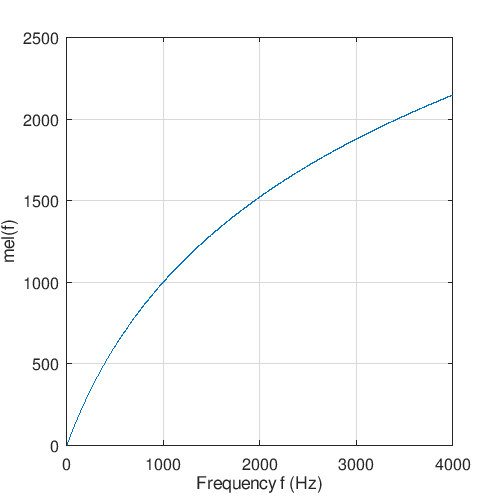
\includegraphics[width=8cm]{ratek_mel_fhz}
\end{center}
\end{figure}

We wish to use $mel(f)$ to construct $warp(k,K)$, such that there are $K$ evenly spaced points on the $mel(f)$ axis (Figure \ref{fig:mel_k}).  Solving for the equation of a straight line we can obtain $mel(f)$ as a function of $k$, and hence $warp(k,K)$ (Figure \ref{fig:warp_fhz_k}):
\begin{equation}
\label{eq:mel_k}
\begin{split}
g &= \frac{mel(3700)-mel(200)}{K-1} \\
mel(f) &= g(k-1) + mel(200)
\end{split}
\end{equation}
where $g$ is the gradient of the line. Substituting (\ref{eq:f_mel}) into the LHS:
\begin{equation}
\label{eq:warp}
\begin{split}
2595log_{10}(1+f/700) &= g(k-1) + mel(200) \\
f_k = warp(k,K) &= mel^{-1} ( g(k-1) + mel(200) ) \\
\end{split}
\end{equation}
and the inverse warp function:
\begin{equation} \label{warp_inv}
k = warp^{-1}(f,K) = \frac{mel(f)-mel(200)}{g} + 1
\end{equation}

\begin{figure}[h]
\caption{Linear mapping of $mel(f)$ to Rate $K$ sample index $k$}
\vspace{5mm}
\label{fig:mel_k}
\centering
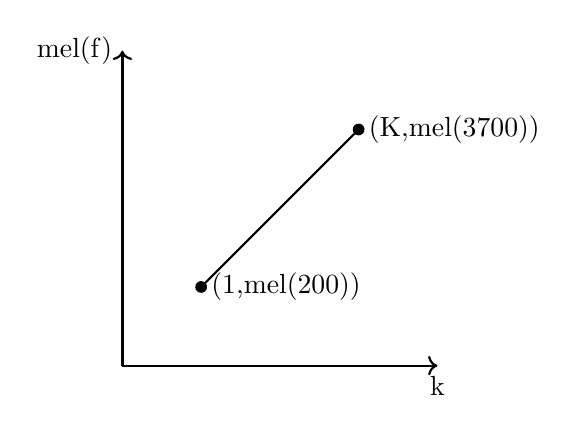
\begin{tikzpicture}
\tkzDefPoint(1,1){A}
\tkzDefPoint(3,3){B}
\draw[thick] (1,1) node [right]{(1,mel(200))} -- (3,3) node [right]{(K,mel(3700))};
\draw[thick,->] (0,0) -- (4,0) node [below]{k};
\draw[thick,->] (0,0) -- (0,4) node [left]{mel(f)};
\foreach \n in {A,B}
  \node at (\n)[circle,fill,inner sep=1.5pt]{};
\end{tikzpicture}
\end{figure}

\begin{figure}[h]
\caption{$warp(k,K)$ function for $K=20$}
\label{fig:warp_fhz_k}
\begin{center}
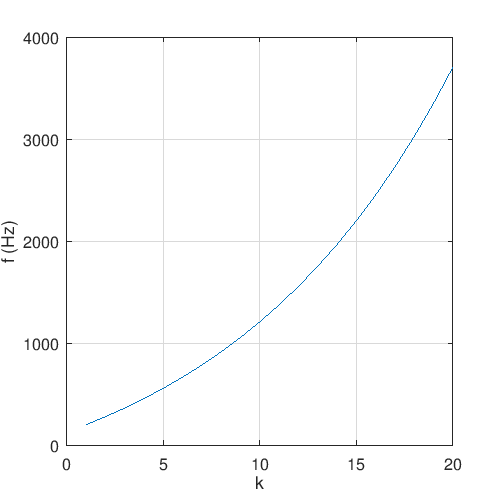
\includegraphics[width=8cm]{warp_fhz_k}
\end{center}
\end{figure}

The input speech may be subject to arbitrary filtering, for example due to the microphone frequency response, room acoustics, and anti-aliasing filter.  This filtering is fixed or slowly time varying.  The filtering biases the target vectors away from the VQ training material, resulting in significant additional mean square error.  The filtering does not greatly affect the input speech quality, however the VQ performance distortion increases and the output speech quality is reduced.  This is exacerbated by operating in the log domain, the VQ will try to match very low level, perceptually insignificant energy near 0 and 4000 Hz. A microphone equaliser algorithm has been developed to help adjust to arbitrary microphone filtering.

For every input frame $l$, the equaliser (EQ) updates the dimension $K$ equaliser vector $\mathbf{e}$:
\begin{equation}
\mathbf{e}^{l} = \mathbf{e}^{l-1} + \beta(\mathbf{b} - \mathbf{t})
\end{equation}
where $\mathbf{t}$ is a fixed target vector set to the mean of the VQ quantiser, and $\beta$ is a small adaption constant.

The equalised, mean removed rate $K$ vector $\mathbf{d}$ is vector quantised for transmission over the channel:
\begin{equation}
\begin{split}
\mathbf{c} &= \mathbf{b} - \mathbf{e} \\
\mathbf{d} &= \mathbf{c} - \bar{\mathbf{c}} \\
\hat{\mathbf{c}} &= VQ(\mathbf{d}) + Q(\bar{\mathbf{c}}) \\
                 &= \hat{\mathbf{d}} + \hat{\bar{\mathbf{c}}}
\end{split}
\end{equation}
Codec 2 700C uses a two stage VQ with 9 bits (512 entries) per stage. The \emph{mbest} multi-stage search algorithm is used to jointly search the two stages (using 5 survivors from the first stage).  Note that VQ is performed in the $log$ amplitude (dB) domain. The mean of $\mathbf{c}$ is removed prior to VQ and scalar quantised and transmitted separately as the frame energy. At the decoder, the rate $L$ vector $\hat{\mathbf{a}}$ can then be recovered by resampling $\mathbf{\hat{a}}$:
\begin{equation}
\hat{\mathbf{a}} = S(\hat{\mathbf{c}} + \mathbf{p})
\end{equation}
where $\mathbf{p}$ is a post filter vector. The post filter vector is generated from the mean-removed rate $K$ vector $\hat{\mathbf{d}}$ in the $log$ frequency domain:
\begin{equation}
\begin{split}
\mathbf{p} &= G + P_{gain} \left( \hat{\mathbf{d}} + \mathbf{r} \right) - \mathbf{r} \\
\mathbf{r} &= \begin{bmatrix} R_1, R_2, \ldots R_K \end{bmatrix} \\
       R_k &= 20log_{10}(f_k/300) \quad k=1,...,K 
\end{split}
\end{equation}
where $G$ is an energy normalisation term, and $1.2 < P_{gain} < 1.5$ describes the amount if post filtering applied.  $G$ and $P_{gain}$ are similar to $g$ and $\beta$ in the LPC/LSP post filter (\ref{eq:lpc_lsp_pf}).  The $\mathbf{r}$ term is a high pass (pre-emphasis) filter with +20 dB/decade gain after 300 Hz ($f_k$ is given in (\ref{eq:warp})).  The post filtering is applied on the pre-emphasised vector, then the pre-emphasis is removed from the final result.  Multiplying by $P_{gain}$ in the $log$ domain is similar to the $\alpha$ power function in (\ref{eq:lpc_lsp_pf}); spectral peaks are moved up, and troughs pushed down.  This filter enhances the speech quality but also introduces some artefacts.

Figure \ref{fig:decoder_newamp1} is the block diagram of the decoder signal processing.  Cepstral techniques are used to synthesise a  phase spectra $arg[H(e^{j \omega}])$ from $\hat{\mathbf{a}}$ using a minimum phase model.  

\begin{figure}[h]
\caption{Codec 2 700C (newamp1) Decoder}
\label{fig:decoder_newamp1}
\begin{center}
\begin{tikzpicture}[auto, node distance=3cm,>=triangle 45,x=1.0cm,y=1.0cm,align=center]

\node [input] (rinput) {};
\node [block, right of=rinput,node distance=1.5cm] (unpack) {Unpack};
\node [block, right of=unpack,node distance=2.5cm] (interp) {Interpolate};
\node [block, right of=interp,node distance=3cm,text width=2cm] (post) {Post Filter};
\node [block, below of=post,text width=2cm,node distance=2cm] (resample) {Resample to Rate $L$};
\node [block, below of=resample,text width=2cm,node distance=2cm] (synth) {Sinusoidal\\Synthesis};
\node [tmp, below of=resample,node distance=1cm] (z1) {};
\node [block, left of=synth,text width=2cm] (phase) {Phase Synthesis};
\node [output,right of=synth,node distance=2cm] (routput) {};

\draw [->] node[align=left,text width=2cm] {Bit\\Stream} (rinput) -- (unpack);
\draw [->] (unpack) -- (interp);
\draw [->] (interp) -- node[above] {$\hat{\mathbf{c}}$} (post);
\draw [->] (post) -- node[left] {$\hat{\mathbf{c}} + \mathbf{p}$} (resample);
\draw [->] (interp) |- node[left] {$\hat{\omega_0}, v$} (resample);
\draw [->] (resample) -- node[right] {$\hat{\mathbf{a}}$}  (synth);
\draw [->] (resample) -- (z1) -| (phase);
\draw [->] (phase) -- (synth);
\draw [->] (synth) -- (routput) node[align=right,text width=1.5cm] {$\hat{s}(n)$};

\end{tikzpicture}
\end{center}
\end{figure}

Some notes on the Codec 2 700C \emph{newamp1} algorithms:
\begin{enumerate}
\item The amplitudes and Vector Quantiser (VQ) entries are in dB, which matches the ears logarithmic amplitude response. 
\item The mode is capable of communications quality speech and is in common use with FreeDV, but is close to the lower limits of intelligibility, and doesn't do well in some languages (problems have been reported with German and Japanese).
\item The VQ was trained on just 120 seconds of data - way too short.
\item The parameter set (pitch, voicing, log spectral magnitudes) is very similar to that used for the latest neural vocoders.
\item The Rate K algorithms were recently revisited, several improvements were proposed and prototyped \cite{rowe2023ratek}.
\end{enumerate}

\section{Summary of Codec 2 Modes}
\label{sect:codec2_modes}

\begin{table}[H]
\label{tab:codec2_modes}
\centering
\begin{tabular}{p{0.75cm}|p{0.75cm}|p{0.5cm}|p{0.5cm}|p{0.5cm}|p{0.5cm}|p{0.5cm}|p{3cm}}
\hline
Mode & Frm (ms) & Bits & $A_m$ & $E$ & $\omega_0$ & $v$ & Use Cases \\
\hline
3200 & 20 & 64 & 50 & 5  & 7  & 2 & M17 \\
2400 & 20 & 50 & 36 & 8  & -  & 2 \\
1600 & 40 & 64 & 36 & 10 & 14 & 4 & M17 \\
1400 & 40 & 56 & 36 & 16 & -  & 4 \\
1300 & 40 & 52 & 36 & 5  & 7  & 4 & FreeDV 1600 \\
1200 & 40 & 48 & 27 & 16 & -  & 4 & \\
700C & 40 & 28 & 18 & 4  & 6  & - & FreeDV 700C/D/E \\
\hline
\end{tabular}
\caption{Codec 2 Modes}
\end{table}

The 3200 mode quantises the LSP differences $\omega_{i+1}-\omega_i$, which provides low distortion at the expense of robustness to bit errors, as an error in a low order LSP difference will propagate through the frame.  The 2400 and 1200 bit/s modes use a joint delta $\omega_0$ and energy VQ, which is efficient but also also suffers from error propagation so is not suitable for high BER use cases.

There is an unfortunate overlap in the naming conventions of Codec 2 and FreeDV.  The Codec 2 700C mode is used in the FreeDV 700C, 700D, and 700E modes.

\section{Summary of Codec 2 Source Files}
\label{sect:source_files}

Codec 2 is part of the \emph{codec2} repository, which also includes various modems and FreeDV API code.  This sections lists the files specific to the speech codec. The \emph{cmake} system builds the \emph{libcodec2} library, which is called by user applications via the Codec 2 API in \emph{codec2.h}.  See the repository \emph{README} for information on building, demo applications, and an introduction to other features of the \emph{codec2} repository.
 
\begin{table}[H]
\label{tab:codec2_file}
\centering
\begin{tabular}{l l}
\hline
File & Description \\
\hline
c2dec & Sample decoder application \\
c2enc & Sample encoder application \\
c2sim & Simulation and development application \\
codebook & Directory containing quantiser tables \\
codec2.c & Quantised encoder and decoder functions that implement each mode \\
codec2\_fft.c & Wrapper for FFT (usually kiss FFT) \\
defines.h & Constants \\
lpc.c & LPC functions \\
mbest.c & Multistage VQ search \\
newamp1.c & Codec 2 700C \emph{newamp1} mode \\
nlp.c & Non-linear Pitch (NLP) \\
sine.c & Sinusoidal analysis, synthesis, voicing estimation \\
phase.c & Phase synthesis \\
quantise.c & Quantisation, in particular for LPC/LSP modes \\
\hline
\end{tabular}
\caption{Codec 2 Source Files}
\end{table}

\section{Glossary}
\label{sect:glossary}

\begin{table}[H]
\label{tab:acronyms}
\centering
\begin{tabular}{l l l }
\hline
Acronym & Description \\
\hline
DFT & Discrete Fourier Transform \\
DTCF & Discrete Time Continuous Frequency Fourier Transform \\
EQ & (microphone) Equaliser \\
IDFT & Inverse Discrete Fourier Transform \\
LPC & Linear Predictive Coding \\
LSP & Line Spectrum Pair \\
MBE & Multi-Band Excitation \\
MSE & Mean Square Error \\
NLP & Non Linear Pitch (algorithm) \\
VQ & Vector Quantiser \\
\hline
\end{tabular}
\caption{Glossary of Acronyms}
\end{table}

\begin{table}[H]
\label{tab:symbol_glossary}
\centering
\begin{tabular}{l l l }
\hline
Symbol & Description & Units \\
\hline
$A(z)$ & LPC (analysis) filter \\
$a_m$ & Lower DFT index of current band \\
$b_m$ & Upper DFT index of current band \\
$\{A_m\}$ & Set of harmonic magnitudes $m=1,...L$ & dB \\
$\mathbf{a}$ & $\{A_m\}$ in vector form \\
$B_m$ & Complex spectral amplitudes used for voicing estimation \\
$E$ & Frame energy \\
$E(z)$ & Excitation in source-filter model \\
$F_0$ & Fundamental frequency (pitch) & Hz \\
$F_s$ & Sample rate (usually 8 kHz) & Hz \\
$F_w(k)$ & DFT of squared speech signal in NLP pitch estimator \\
$G$ & LPC gain \\
$H(z)$ & Synthesis filter in source-filter model \\
$\hat{H}(z)$ & Synthesis filter approximation after quantisation \\
$l$ & Frame index \\
$L$ & Number of harmonics \\
$N$ & Processing frame size in samples \\
$n_0$ & Excitation pulse position \\
$P$ & Pitch period & ms or samples \\
$P(z), Q(z)$ & LSP polynomials \\
$P_f(e^{j \omega})$ & LPC post filter \\
$\{\theta_m\}$ & Set of harmonic phases $m=1,...L$ & dB \\
$r$ & Maps a harmonic number $m$ to a DFT index \\
$s(n)$ & Input time domain speech \\
$\hat{s}(n)$ & Output (synthesised) time domain speech \\
$s_w(n)$ & Time domain windowed input speech \\
$S_w(k)$ & Frequency domain windowed input speech \\
$\hat{S}_w(k)$ & Frequency domain output (synthesised)speech \\
$t(n)$ & Triangular synthesis window \\
$\phi_m$ & Phase of excitation harmonic \\
$\omega_0$ & Fundamental frequency (pitch) & radians/sample \\
$\{\omega_i\}$ & Set of LSP frequencies \\
$w(n)$ & Window function \\
$W(k)$ & DFT of window function \\
$v$ & Voicing decision for the current frame \\
\hline
\end{tabular}
\caption{Glossary of Symbols}
\end{table}

\section{Further Documentation Work}
\label{sect:further_work}

This section contains ideas for expanding the documentation of Codec 2.  Please contact the authors if you are interested in this material or would like to help develop it.

\begin{enumerate}
\item The \emph{c2sim} utility is presently undocumented. We could add some worked examples aimed at the experimenter - e.g. using c2sim to extract and plot model parameters.  Demonstrate how to listen to various stages of quantisation.
\item Several GNU Octave scripts exist that were used to develop Codec 2. We could add information describing how to use the Octave tools to single step through the codec operation.
\end{enumerate}

\addcontentsline{toc}{chapter}{References}
\bibliographystyle{plain}
\bibliography{codec2_refs}
\end{document}
